\documentclass{beamer}

\usepackage[utf8x]{inputenc}
\usepackage[T1]{fontenc}
\usepackage[ngerman]{babel}
\usepackage{helvet}
\usepackage{tikz}
\usepackage{cancel}
\usetikzlibrary{positioning,shapes,calc}

\includeonly{
    metadata,
    content
}

\usetheme{Goettingen}
\setbeamertemplate{headline}[default]
\makeatletter
\setbeamertemplate{sidebar \beamer@sidebarside}{
    \beamer@tempdim=\beamer@sidebarwidth%
    \advance\beamer@tempdim by -6pt%
    {\usebeamerfont{title in sidebar}%
      \vskip1.5em%
      \hskip3pt%
      \usebeamercolor[fg]{title in sidebar}%
      \insertshorttitle[width=\beamer@tempdim,center,respectlinebreaks]\par%
      \vskip1.25em%
    }%
    {%
      \hskip3pt%
      \usebeamercolor[fg]{author in sidebar}%
      \usebeamerfont{author in sidebar}%
      \insertshortauthor[width=\beamer@tempdim,center,respectlinebreaks]\par%
      \vskip1.25em%
    }%
    \insertverticalnavigation{\beamer@sidebarwidth}%
    \vfill
    {\usebeamerfont{section in sidebar}%
      \usebeamercolor[fg]{section in sidebar}%
      \parbox[][\baselineskip][t]{\beamer@sidebarwidth}{%
        \centering%
        \insertframenumber~/~\inserttotalframenumber%
      }%
      \vskip1ex%
    }%
    \ifx\beamer@sidebarside\beamer@lefttext%
    \else%
      \usebeamercolor{normal text}%
      \llap{\usebeamertemplate***{navigation symbols}\hskip0.1cm}%
      \vskip2pt%
    \fi%
}
\makeatother
\AtBeginSection[]
{
 \begin{frame}
  \frametitle{Fahrplan}
  \tableofcontents[currentsection,hideothersubsections]
 \end{frame}
}



\newcommand{\dcsubject}{Chaos Computer Club M"unchen e.V., FifF e.V., JFF - Jugend Film Fernsehen e.V.}
\newcommand{\dctitle}{Cryptoparty}
\newcommand{\dcsubtitle}{Introduction}

\newcommand{\dcauthors}{Michael Weiner, Florian Wilde}
\newcommand{\dcdate}{\today}

\newcommand{\dcplace}{, München}

\newcommand{\dckeywords}{Cryptoparty CCC München}

\hypersetup{
    pdftitle = {\dctitle},
    pdfsubject = {\dcsubject, \dcdate},
    pdfauthor = {\dcauthors},
    pdfkeywords = {\dckeywords},
    pdfcreator = {pdfTeX with Hyperref},
    pdfproducer = {LaTeX, hyperref},
}



\title{\dctitle}
\author{\dcauthorsshort}
\date{\dcdate}

% Placeholder for the email.tex section, content will be defined there
\newcommand{\emailtext}{}
\newcommand{\emailciphertext}{}
\newlength{\messagewidth}

% For blocks that contain only items
\newenvironment{blit}[1]{%
\begin{block}{#1}
\begin{itemize}
}{%
\end{itemize}
\end{block}
}

\newenvironment{blex}[1]{%
\begin{block}{#1}
\begin{description}
}{%
\end{description}
\end{block}
}

\begin{document}

{%
\setbeamertemplate{background}{}
\begin{frame}[plain]
  \titlepage

  \vfill
  \begin{flushright}
    \href{https://creativecommons.org/licenses/by-sa/4.0/}{
\includegraphics[height=3ex]{images/by-sa.png}}
  \end{flushright}
\end{frame}
}

\begin{frame}
\frametitle{Fahrplan}
\tableofcontents[hidesubsections]
\end{frame}

\section{Über den Veranstalter und Cryptopartys}
\begin{frame}{Veranstalter}
  \begin{itemize}
    \item Chaos Computer Club München e.V.
    \item Forum InformatikerInnen für Frieden\\und gesellschaftliche Verantwortung e.V.
    \item Medienzentrum München (MZM)\\Institut für Medienpädagogik in Forschung und Praxis\\JFF -- Jugend Film Fernsehen e.V.
  \end{itemize}
\end{frame}

\endinput

\section{Grundlegendes}
\begin{frame}{Warnhinweise}
  \begin{itemize}
    \item 100\% Sicherheit gibt es nicht
    \item Absichern heißt, Angriffe \emph{teurer} zu machen
    \begin{itemize}
    \item Die Kosten für den Angriff\\ müssen den Wert der Daten übersteigen
    \item Ein Angriff darf sich nicht mehr \emph{lohnen}
    \item Problem: Wert wird oft unterschätzt
    \end{itemize}
    \item Was wir hier zeigen, ist ein Anfang
    \begin{itemize}
      \item Hilft dagegen, als ,,Beifang`` zu enden
      \item Gegen gezielte Angriffe -- auch durch Verwechslung -- benötigt es deutlich mehr
    \end{itemize}
    \item Irren ist menschlich -- auch was die Inhalte der folgenden Folien betrifft :-)
  \end{itemize}
\end{frame}

\begin{frame}{Leitfragen}
  \begin{itemize}
    \item \emph{Was} soll sichergestellt werden?
      \begin{itemize}
        \item Eigene Anonymität
        \item Echtheit des Gegenübers (Authentizität)
        \item Unverfälschtheit der Nachricht (Integrität)
        \item Geheimhaltung der Nachricht (Vertraulichkeit)
        \item \ldots
      \end{itemize}
    \item \emph{Wem} vertraut Ihr?
  \end{itemize}
\end{frame}

\begin{frame}{Vertrauen}
  \begin{block}{Woher weiß man, wem man vertrauen kann?}
  \begin{itemize}
    \item Kurze Antwort: weiß man \emph{nicht}
    \item Lange Antwort
    \begin{itemize}
      \item es gibt Fragen, die man stellen kann\ldots
      \item \ldots\ und es gibt das Bauchgefühl
    \end{itemize}
  \end{itemize}
  \end{block}
\end{frame}

\begin{frame}{Welche Fragen kann man stellen?}
  Beispiel: \emph{Wo} sind meine Daten?
  \begin{itemize}
    \item Auf einem Blatt Papier zuhause in meiner Schublade.
    \item Auf meinem Computer:
    \begin{itemize}
      \item Wie gut ist die Software \emph{überprüfbar},\\ die meine Daten verwaltet?
      \begin{itemize}
        \item Open Source (in menschenlesbarer Form öffentlich):\\gut überprüfbar
        \item Closed Source (menschenlesbare Form geheim):\\quasi nicht überprüfbar
      \end{itemize}
    \end{itemize}
    \item In der Cloud
      %TODO: FSF there is no cloud
      \begin{itemize}
        \item \emph{Wer} betreibt einen Dienst?
        \item Womit \emph{verdient} der Betreiber sein \emph{Geld}?
        \item Wem könnten die Daten \emph{nutzen} oder \emph{schaden}?
        \item Was \emph{lernt} der Betreiber über mich?
      \end{itemize}
  \end{itemize}
\end{frame}

\begin{frame}{Meta- und Nutzdaten}
  \begin{itemize}
    \item Meta-/Verbindungsdaten (``Briefumschlag'')
    \begin{itemize}
      \item Absender, Empfänger, Betreff einer E-Mail
      \item Besuch und Aufenthaltsdauer auf einer Webseite
      \item Wer, wann, wie lange mit wem telefoniert
      \item Aufenthaltsort von Mobiltelefonen: Bewegungsprofil!
    \end{itemize}
    \item Nutz-/Inhaltsdaten (``Brief'')
    \begin{itemize}
      \item E-Mail-Text und -Anhänge
      \item Webseiten-Inhalte
      \item Gesprochene Sprache beim Telefonieren
      \item SMS-Inhalt
    \end{itemize}
  \end{itemize}

Metadaten zu verschlüsseln ist nicht möglich,\\ sie zu verschleiern schwierig.
\end{frame}


\endinput

\section{Passwörter}
\begin{frame}{Passwörter}
  \visible<+->{Wer hat mindestens fünf Online-Accounts?}

  \visible<+->{Wer hat dafür mindestens drei verschiedene Passwörter?}

  \visible<+->{Wer beachtet, Passwörter nur über HTTPS einzugeben?}
\end{frame}

\begin{frame}{Anzahl Passwörter}
  \begin{itemize}
    \item Kundendaten gehen häufig verloren
    \begin{itemize}
      \item Schaden lässt sich begrenzen, wenn Benutzername und Passwort nur bei diesem einen Anbieter passen
    \end{itemize}
    \item Besonder wichtig: E-Mail-Accounts
    \begin{itemize}
      \item Weil ,,Passwort zurücksetzen`` oft via E-Mail
      \item Wer den E-Mail Account übernommen hat,\\ kann dadurch sämtliche Accounts übernehmen
    \end{itemize}
    \item Ideal: Jedes Passwort nur einmal verwenden
    \item Alternative: Passwörter ,,salzen``
    \begin{itemize}
      \item \textit{passwort}.amz für Onlineshop a
      \item \textit{passwort}.zal für Onlineshop z
      \item \textit{anderespasswort} für Mails
    \end{itemize}
  \end{itemize}
\end{frame}

\begin{frame}{Sichere Passwörter}
  \begin{block}{Anforderungen}
  \begin{itemize}
    \item Klein- und Großbuchstaben, Zahlen,\\ begrenzt: Sonderzeichen
    \item Wichtiger: Lang genug!
  \end{itemize}
  \end{block}
  \begin{block}{Merkbarkeit}
  \begin{itemize}
    \item Geschichte dazu ausdenken
    \item Melodie und Rhythmus rein bringen
    \begin{itemize}
      \item Gehirn kann sich Melodien besonders leicht merken
      \item Ermöglicht schnelles Eintippen
      \begin{itemize}
        \item Längere Passwörter sind weniger nervig
        \item Passwort mitlesen ist schwieriger
      \end{itemize}
    \end{itemize}
  \end{itemize}
  \end{block}
\end{frame}

\begin{frame}{Passwort Länge vs. Zeichensatz}
  \begin{center}
    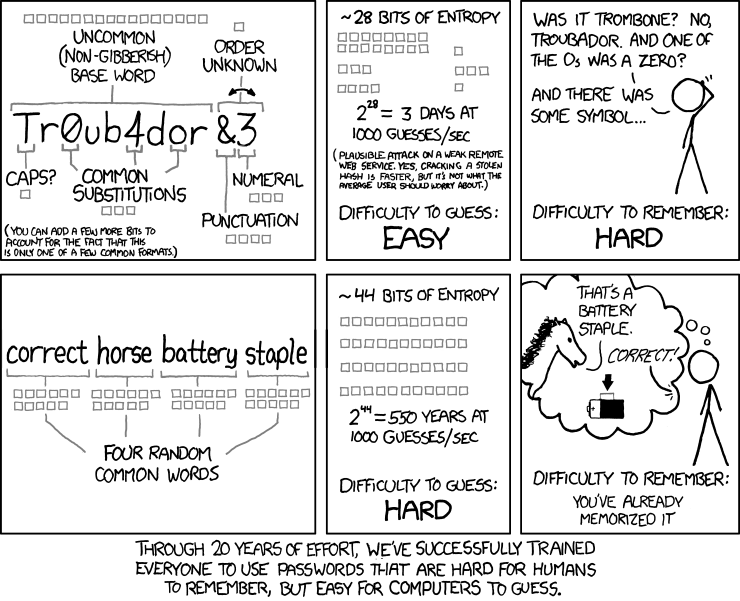
\includegraphics[width=0.99\textheight]{images/password_strength.png}\\
  \end{center}
  \tiny Bildquelle: \href{http://xkcd.com/936/}{xkcd: Password Strength / CC BY-NC 2.5}
\end{frame}

\begin{frame}{Passwort-Manager}
  \begin{itemize}
    \item Software zur Verwaltung von Passwörtern
    \item Kann automatisch komplexe Passwörter erzeugen
    \item Datenbank wird mit Master-Passwort verschlüsselt
    \begin{itemize}
      \item Anzahl der zu merkenden Passwörter geringer
    \end{itemize}
    \item Beispiel: KeePassX (Open Source)
  \end{itemize}
    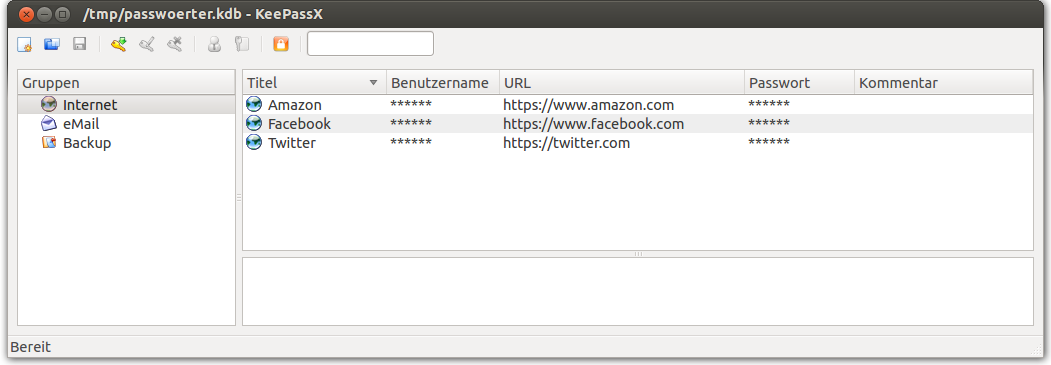
\includegraphics[width=\textwidth]{images/keepassx.png}
  \begin{itemize}
    \item \emph{Wichtige Passwörter trotzdem merken!}
    \item \ldots oder zumindest auf einem Zettel aufschreiben\\ und zuhause an einem sicheren Ort lagern
  \end{itemize}
\end{frame}

\endinput

\section{Web-Surfen}
\begin{frame}{Tracking}
  \begin{itemize}
    \item Cookies und Co (HTML5 Persistent Local Storage, Flashcookies, \ldots)
    \item Browser-Fingerabdruck
    \item IP-Adresse
  \end{itemize}
  Jede Website und jedes Werbenetzwerk\\kann Personen und Computer (wieder-)erkennen

  \begin{block}{Tools zur Aufklärung}
  \begin{itemize}
    \item \href{https://panopticlick.eff.org/}{EFF: Panopticlick}
    \item \href{http://datenblumen.wired.de/}{Wired: Datenblumen}
  \end{itemize}
  \end{block}
\end{frame}

\begin{frame}{Schutzmaßnahmen -- Level 1}
\framesubtitle{Nur Einstellungen ändern}
  \begin{itemize}
    \item Standardsuchmaschine\\ auf datenschutzfreundliche Anbieter ändern, z.B.
    \begin{itemize}
      \item DuckDuckGo
      \item Startpage
    \end{itemize}
    \item Cookies verbieten, nur selektiv erlauben
    \begin{itemize}
      \item Firefox: about:preferences
    \end{itemize}
    \item Plugins auf ,,Click-to-use`` stellen
    \begin{itemize}
      \item Firefox: about:addons
    \end{itemize}
    \item Wer möchte: Verlauf beim Beenden löschen
  \end{itemize}

  Eventuell:
  \begin{itemize}
    \item Blockierung von ,,bösen`` Webseiten abschalten
    \item Statusberichte des Browsers abschalten
  \end{itemize}
\end{frame}

\begin{frame}{Schutzmaßnahmen -- Level 2}
\framesubtitle{Plug-Ins installieren}
  \begin{itemize}
    \item Adblocker --\\ Schadsoftware immer öfter über Werbeanzeigen!
    \begin{itemize}
      \item uBlock origin
      \begin{itemize}
        \item Keine \glqq acceptable adds\grqq\ wie bei Adblock Plus
        \item Blockiert auch andere nervige Dinge außer Werbung
      \end{itemize}
      \item \href{https://www.eff.org/privacybadger}{EFF: Privacy Badger}
      \begin{itemize}
        \item Blockiert anhand von Verhalten, nicht Listen
      \end{itemize}
      %\item TODO: RequestPolicy
    \end{itemize}
    \item NoScript
    \begin{itemize}
      \item Erlaubt gezieltes ein-/ausschalten von Java, JavaScript etc.
    \end{itemize}
    \item EFF: HTTPS-Everywhere
    \begin{itemize}
      \item Nutzt automatisch HTTPS, falls von Seite unterstützt
      \item Benutzt lokale Liste der Seiten, keine Online-Abfrage
    \end{itemize}
    \item RefControl
    \begin{itemize}
      \item HTTP-Referrer = von welcher Seite komme ich
    \end{itemize}
  \end{itemize}
\end{frame}

\begin{frame}{Schutzmaßnahmen -- Level 3}
\framesubtitle{Neue Programme installieren oder benutzen}
  \begin{itemize}
    \item \href{https://www.torproject.org}{Tor Browser Bundle (Freie Software)}
    \begin{itemize}
      \item Anonymisierung des Netzwerkverkehrs\\durch \emph{\glqq intelligente Umwege\grqq}
      \item Fingerabdruck bei allen Tor Browsern identisch
      \item Gewählte Plugins vorinstalliert
      \item Automatische Updates, Installation mit einem Klick
      \item Hohe Sicherheit, aber prinzipbedingt langsamer
    \end{itemize}
    \item \href{https://tails.boum.org}{Tails (Freie Software)}
    \begin{itemize}
      \item Abgesichertes Betriebssystem inkl. Tor
      \item Leitet \emph{gesamten} Verkehr über Tor
      \item Live System = kann direkt von CD gebootet werden\\ hinterlässt keinerlei Spuren am PC
      % As of 2016-Apr-14, Windows Camouflage has been removed in Tails 2 and newer
      %   https://tails.boum.org/news/windows_camouflage_jessie/index.en.html
      %   https://tails.boum.org/blueprint/update_camouflage_for_jessie/
      %\item Sieht auf Wunsch nach Windows aus
    \end{itemize}
  \end{itemize}
\end{frame}

\endinput

\section{E-Mail}
\begin{frame}{Was soll geschützt werden?}
  E-Mails können
  \begin{itemize}
    \item abgehört
    \item gefälscht
  \end{itemize}
  werden. \pause Deshalb stellen wir vor, wie man
  \begin{itemize}
    \pause
    \item die Vertraulichkeit (das ,,Briefgeheimnis``) umsetzt
    \\ $\Rightarrow$ Verschlüsselung
    \pause
    \item die Echtheit des Gegenübers sicherstellt
    \\ $\Rightarrow$ Digitale Signatur
  \end{itemize}
  \pause
  \vfill
  Außerdem:\\ Wie man sicherstellt, dass das E-Mail Passwort\\ nicht einfach mitgelesen werden kann
\end{frame}

\renewcommand{\emailtext}{Von: Alice@provider1.de\\An: Bob@provider2.com\\Betreff: Hallo\\Hallo Bob, wie gehts dir?\\LG Alice}
\renewcommand{\emailciphertext}{Von: Alice@provider1.de\\An: Bob@provider2.com\\Betreff: Hallo\\\colorbox{blue}{\parbox[t][1.2em][t]{.88\messagewidth}{~}}}
\settowidth{\messagewidth}{\tiny Hallo Bob, wie gehts dir?}
\addtolength{\messagewidth}{3\pgfkeysvalueof{/pgf/outer xsep}}

\begin{frame}{Funktionsweise}
  \framezoom<1><2>(-0.3cm,0cm)(3cm,4.5cm)
  \framezoom<1><3>(4.5cm,0cm)(3cm,4.5cm)
  \begin{center}\tiny
  \begin{tikzpicture}[align=left]
    \tikzstyle{attacker} = [draw,circle]
    \tikzstyle{entity} = [draw,rectangle split,rectangle split parts=2]
    \tikzstyle{message} = [fill=white,text width=\messagewidth]
      \node[attacker] (eve) at (0,0) {Eve};
      \node[entity] (alice) at (-3.75cm,2.5cm) {Alice\nodepart{second}\emailtext};
      \node[entity] (Palice) at (-3.75cm,-2.0cm) {provider1.de\nodepart{second}\emailtext};
      \node[entity] (Pbob) at (3.75cm,-2.0cm) {provider2.com\nodepart{second}\emailtext};
      \node[entity] (bob) at (3.75cm,2.5cm) {Bob\nodepart{second}\emailtext};
      \draw[->] (alice) -- (Palice) node [pos=0.25,message] (aliceHello) {Hier ist Alice, mein Passwort ist AAA. Ich will eine E-Mail verschicken:} node [pos=0.70,message] (aliceSend) {\emailtext};
      \draw[->] (Palice) -- (Pbob) node [midway,message] (providerFwd) {\emailtext};
      \draw[<->] (bob) -- (Pbob) node [pos=0.25,message] (bobHello) {Hier ist Bob, mein Passwort ist BBB. Gib mir meine neuen E-Mails!} node [pos=0.70,message] (bobReceive) {\emailtext};
      \foreach \t in {(aliceHello),(aliceSend),(Palice),(providerFwd),(Pbob),(bobHello),(bobReceive)} \draw[->,red,thick] (eve) -- \t;
      \draw[dashed,red] ($ (alice.south west)!.5!(aliceHello.north west) $) -- ($ (bob.south east)!.5!(bobHello.north east) $);
  \end{tikzpicture}
  \end{center}
  \vspace{-1em}
  \begin{itemize}
    \item \glqq Von\grqq\ und \glqq An\grqq\ kann Absender beliebig setzen,\\ wie auf einem Briefumschlag!
  \end{itemize}
\end{frame}

\begin{frame}{Transportverschlüsselung}{SSL/TLS, besser STARTTLS}
  \begin{center}\tiny
  \begin{tikzpicture}[align=left]
    \tikzstyle{attacker} = [draw,circle]
    \tikzstyle{entity} = [draw,rectangle split,rectangle split parts=2]
    \tikzstyle{message} = [fill=yellow,text=yellow,text width=\messagewidth]
      \node[attacker] (eve) at (0,0) {Eve};
      \node[entity] (alice) at (-3.75cm,2.5cm) {Alice\nodepart{second}\emailtext};
      \node[entity] (Palice) at (-3.75cm,-2.0cm) {provider1.de\nodepart{second}\emailtext};
      \node[entity] (Pbob) at (3.75cm,-2.0cm) {provider2.com\nodepart{second}\emailtext};
      \node[entity] (bob) at (3.75cm,2.5cm) {Bob\nodepart{second}\emailtext};
      \draw[->] (alice) -- (Palice) node [pos=0.25,message] (aliceHello) {Hier ist Alice, mein Passwort ist AAA. Ich will eine E-Mail verschicken:} node [pos=0.70,message] (aliceSend) {\emailtext};
      \draw[->] (Palice) -- (Pbob) node [midway,message] (providerFwd) {\emailtext};
      \draw[<->] (bob) -- (Pbob) node [pos=0.25,message] (bobHello) {Hier ist Bob, mein Passwort ist BBB. Gib mir meine neuen E-Mails!} node [pos=0.70,message] (bobReceive) {\emailtext};
      \foreach \t in {(aliceHello),(aliceSend),(Palice),(providerFwd),(Pbob),(bobHello),(bobReceive)} \draw[->,red,thick] (eve) -- \t;
      \draw[dashed,red] ($ (alice.south west)!.5!(aliceHello.north west) $) -- ($ (bob.south east)!.5!(bobHello.north east) $);
  \end{tikzpicture}
  \end{center}
  \vspace{-1em}
  \begin{itemize}
    \item Inzwischen von fast allen Mailanbietern unterstützt
    \item Konfiguration des Mailprogramms überprüfen!
  \end{itemize}
\end{frame}

\begin{frame}{Ende-zu-Ende-Verschlüsselung}{OpenPGP, S/MIME}
  \begin{center}\tiny
  \begin{tikzpicture}[align=left]
    \tikzstyle{attacker} = [draw,circle]
    \tikzstyle{entity} = [draw,rectangle split,rectangle split parts=2]
    \tikzstyle{message} = [fill=white,text width=\messagewidth]
      \node[attacker] (eve) at (0,0) {Eve};
      \node[entity] (alice) at (-3.75cm,2.5cm) {Alice\nodepart{second}\emailtext};
      \node[entity] (Palice) at (-3.75cm,-2.0cm) {provider1.de\nodepart{second}\emailciphertext};
      \node[entity] (Pbob) at (3.75cm,-2.0cm) {provider2.com\nodepart{second}\emailciphertext};
      \node[entity] (bob) at (3.75cm,2.5cm) {Bob\nodepart{second}\emailtext};
      \draw[->] (alice) -- (Palice) node [pos=0.25,message] (aliceHello) {Hier ist Alice, mein Passwort ist AAA. Ich will eine E-Mail verschicken:} node [pos=0.70,message] (aliceSend) {\emailciphertext};
      \draw[->] (Palice) -- (Pbob) node [midway,message] (providerFwd) {\emailciphertext};
      \draw[<->] (bob) -- (Pbob) node [pos=0.25,message] (bobHello) {Hier ist Bob, mein Passwort ist BBB. Gib mir meine neuen E-Mails!} node [pos=0.70,message] (bobReceive) {\emailciphertext};
      \foreach \t in {(aliceHello),(aliceSend),(Palice),(providerFwd),(Pbob),(bobHello),(bobReceive)} \draw[->,red,thick] (eve) -- \t;
      \draw[dashed,red] ($ (alice.south west)!.5!(aliceHello.north west) $) -- ($ (bob.south east)!.5!(bobHello.north east) $);
  \end{tikzpicture}
  \end{center}
  \vspace{-1em}
  \begin{itemize}
    \item Unabhängig vom Mailanbieter möglich
    \item Benötigt Zusatzsoftware und Schlüssel bei beiden
  \end{itemize}
\end{frame}

\begin{frame}{Kombination Transport \& Ende-zu-Ende}
  \begin{center}\tiny
  \begin{tikzpicture}[align=left]
    \tikzstyle{attacker} = [draw,circle]
    \tikzstyle{entity} = [draw,rectangle split,rectangle split parts=2]
    \tikzstyle{message} = [fill=yellow,text=yellow,text width=\messagewidth]
      \node[attacker] (eve) at (0,0) {Eve};
      \node[entity] (alice) at (-3.75cm,2.5cm) {Alice\nodepart{second}\emailtext};
      \node[entity] (Palice) at (-3.75cm,-2.0cm) {provider1.de\nodepart{second}\emailciphertext};
      \node[entity] (Pbob) at (3.75cm,-2.0cm) {provider2.com\nodepart{second}\emailciphertext};
      \node[entity] (bob) at (3.75cm,2.5cm) {Bob\nodepart{second}\emailtext};
      \draw[->] (alice) -- (Palice) node [pos=0.25,message] (aliceHello) {Hier ist Alice, mein Passwort ist AAA. Ich will eine E-Mail verschicken:} node [pos=0.70,message] (aliceSend) {\emailtext};
      \draw[->] (Palice) -- (Pbob) node [midway,message] (providerFwd) {\emailtext};
      \draw[<->] (bob) -- (Pbob) node [pos=0.25,message] (bobHello) {Hier ist Bob, mein Passwort ist BBB. Gib mir meine neuen E-Mails!} node [pos=0.70,message] (bobReceive) {\emailtext};
      \foreach \t in {(aliceHello),(aliceSend),(Palice),(providerFwd),(Pbob),(bobHello),(bobReceive)} \draw[->,red,thick] (eve) -- \t;
      \draw[dashed,red] ($ (alice.south west)!.5!(aliceHello.north west) $) -- ($ (bob.south east)!.5!(bobHello.north east) $);
  \end{tikzpicture}
  \end{center}
\end{frame}

\begin{frame}{Authentizität öffentlicher Schlüssel}
Was, wenn A eine Nachricht an B schicken will,\\ aber den öffentlichen Schlüssel von B nicht kennt?\\
\begin{enumerate}
  \item Im ``Telefonbuch'' nach dem Schlüssel suchen
  \item Echtheit mit Hilfe eines \emph{vertrauenswürdigen Dritten} C überprüfen
\end{enumerate}
\begin{center}
  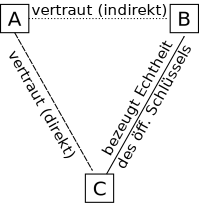
\includegraphics[width=0.5\textheight]{images/vertrauen.pdf}
  %TODO: überarbeiten
\end{center}
\end{frame}

\begin{frame}{Wie stellt man Vertrauen in öffentliche Schlüssel her?}
  \begin{itemize}
    \item S/MIME -- Hierarchischer Vertrauensansatz
    \begin{itemize}
      \item hier nicht behandelt
    \end{itemize}
    \item OpenPGP -- Dezentraler Vertrauensansatz
    \begin{itemize}
      \item jeder kann festlegen, wem er vertraut
      \begin{itemize}
        \item er kann die Echtheit eines Schlüssels\\ z.B. bei einem persönlichen Treffen überprüfen
      \end{itemize}
      \item jeder \emph{kann} sein Vertrauensnetz veröffentlichen (Web-of-Trust)
      \begin{itemize}
        \item Vorteil: Man kann ``Freunden von Freunden'' vertrauen
        \item Nachteil: Beziehungen zwischen Menschen öffentlich\\ Aber: Facebook sagt da viel mehr aus
      \end{itemize}
      %\item wird hier behandelt
    \end{itemize}
  \end{itemize}
\end{frame}

\begin{frame}{Welche Software benötigt man?}
  \begin{block}{OpenPGP Backend}
    Macht die eigentliche Ver-/Entschlüsselung \& Signatur

    \vspace{1ex}
    \begin{tabular}{cccc}
      Linux:            & Windows: & Android:     & Mac:\\
      \emph{schon dabei} & GPG4Win  & OpenKeychain & GPGTools\footnote{kommerziell}\\
    \end{tabular}
  \end{block}
  \begin{block}{Plug-In fürs Mailprogramm}
    Grafische Oberfläche, leichtere Schlüsselverwaltung, etc.

    \vspace{1ex}
    \begin{tabular}{cccc}
      Thunderbird: & Outlook: & K9-Mail:            & Apple Mail:\\
      Enigmail     & GPG4Win  & \emph{integriert} & GPGTools\\
    \end{tabular}
  \end{block}
\end{frame}

\endinput

\section{Messenger}
\begin{frame}{Motivation}
  \begin{itemize}
    \item Komfortabel, auf Smartphone einfach nutzbar
    \item Wird im privaten Umfeld meist häufiger eingesetzt\\ als E-Mail
  \end{itemize}

  \pause
  \begin{block}{Bestandsaufnahme}
    Wer benutzt
    \begin{itemize}
      \item<+-> WhatsApp
      \item<+-> Telegram
      \item<+-> Threema
      \item<+-> Signal
      \item<+-> Jabber
      \item<+-> Matrix
    \end{itemize}
  \end{block}
\end{frame}

\begin{frame}{Überblick}
  \begin{itemize}
    \item Geschlossene Systeme: WhatsApp \& Co
      \begin{itemize}
        \item \emph{Eine Firma} kontrolliert\\ App, Protokoll und ist Dienstanbieter
        \item Auswahl eines Dienstes\\bestimmt erreichbaren Personenkreis
        \item Meist closed-source
      \end{itemize}
    \item Offene Systeme (z.B. Jabber/XMPP, Matrix)
      \begin{itemize}
        \item App, Dienstanbieter und Protokoll kommen\\ von \emph{unterschiedlichen} Firmen bzw. Personen
        \item Alle Nutzer des Protokolls können erreicht werden, egal welche App sie nutzen\\ und bei welchem Dienstanbieter sie sind
        \item Meist open-source
      \end{itemize}
  \end{itemize}
\end{frame}

\setbeamersize{description width=1em}

\begin{frame}{WhatsApp}
  \begin{blex}{Vor- und Nachteile}
    \item[+] Angeblich sehr gute Crypto (von Signal eingekauft)
    \item[+] Verwendbar ohne Google Play Services
    \item[-] Closed-source
    \item[-] Anbieter erhält vollständiges Telefonbuch\\
             (nicht nur WhatsApp-Kontakte)
    \item[-] Metadatenanalyse, -weitergabe an Facebook
  \end{blex}
  \begin{block}{Tipps}
    \begin{itemize}
      \item Ab Android 6 und bei iOS kann man den Zugang zum Telefonbuch sperren
      \item Android 8 Dual Messenger erlaubt\\selektive Freigabe von Kontakten\\
            \scriptsize nicht getestet, nur Samsung(?)
    \end{itemize}
  \end{block}
\end{frame}

\begin{frame}{Telegram}
  \begin{blex}{Vor- und Nachteile}
    \item[+] \glqq Sichere Chats\grqq\ bieten ausreichende Sicherheit
    \item[-] Chats nicht standardmäßig verschlüsselt
    \item[-] Anbieter erhält vollständiges Telefonbuch\\ (nicht nur Telegram-Kontakte)
    \item[-] \glqq Standard-Chats\grqq\ werden im Klartext\\beim Anbieter gespeichert
  \end{blex}
  \begin{block}{Tipps}
    \begin{itemize}
      \item Ab Android 6 und bei iOS kann man den Zugang zum Telefonbuch sperren
    \end{itemize}
  \end{block}
\end{frame}

\begin{frame}{Threema}
  \begin{blex}{Vor- und Nachteile}
    \item[+] Chats hinreichend gut verschlüsselt\\(aber nicht gut überprüfbar, da nicht quelloffen)
    \item[+] Synchronisation des Telefonbuchs optional
    \item[+] Überprüfung der Schlüssel über QR-Code
    \item[o] kostenpflichtig
    \item[-] nicht quelloffen
  \end{blex}
\end{frame}

\begin{frame}{Signal}
  \begin{blex}{Vor- und Nachteile}
    \item[+] Chats standardmäßig sehr gut verschlüsselt
    \item[+] Verwendbar ohne Google Play Services %https://netzpolitik.org/2017/signal-fuer-android-jetzt-ohne-google-play-store/
    \item[+] Überprüfung der Schlüssel über QR-Code
    \item[-] Anbieter erhält komplettes Telefonbuch\\ (nicht nur Signal-Kontakte)
  \end{blex}
  \begin{block}{Tipps}
    \begin{itemize}
      \item Ab Android 6 und bei iOS kann man den Zugang zum Telefonbuch sperren
    \end{itemize}
  \end{block}
\end{frame}

\begin{frame}{Jabber/XMPP}
  \begin{blex}{Vor- und Nachteile}
    \item[+] Offenes System: Anbieter und App frei wählbar
    \item[+] Verschlüsselung möglich (OTR oder OMEMO)
    \item[+] Keine Telefonbuch-Synchronisation vorgesehen
    \item[-] Crypto nicht ganz so nutzerfreundlich\\wie bei kommerziellen Anbietern\\(aber dafür sind wir ja alle hier :-)
  \end{blex}
  \begin{itemize}
    \item Apps: Conversations, pidgin, gajim, \ldots
    \item Anbieter: Unis, Hackerspaces, CCC, jabber.org, \ldots
  \end{itemize}
\end{frame}

\begin{frame}{Matrix}
  \begin{blex}{Vor- und Nachteile}
    \item[+] Offenes System: Anbieter frei wählbar
    \item[+] Verschlüsselung möglich
    \item[+] Telefonbuch-Synchronisation nicht zwingend
    \item[+] Anbindung an Drittsysteme möglich (IRC, Skype, \ldots)
    \item[-] Hintergrund/Historie der Entwickler umstritten
  \end{blex}
\end{frame}

\begin{frame}{Zusammenfassung}
  \begin{itemize}
    \item Viele beliebte Messenger\\ sind geschlossene Systeme
    \item Darauf achten, womit der Anbieter sein Geld verdient
    \item Wer auf bestimmte Messenger nicht verzichten kann: Zugriff auf Kontakte verbieten!
  \end{itemize}
\end{frame}

\section{Fragen, Feedback}
\begin{frame}{Fragen, Feedback, ...}
  \begin{itemize}
    \item{Her damit!}
    \item{Fragen an alle Helfer (bitte gebt Euch zu erkennen :-)}
    \item{Links: \url{https://muc.pads.ccc.de/cryptoparty}}
  \end{itemize}
\end{frame}

\endinput


\end{document}
